\section{Sprint Material} % (fold)
\label{sec:Sprint Material}
\subsection{Version} % (fold)
\label{sub:Version}
The current state of our app has version 0.0.1. Meaning that the app is still alpha quality, with some functionality implementet, but lot of unfinished work.
% subsection Version (end)
\subsection{Source code} % (fold)
\label{sub:Source code}
We still use Git and GitHub. The source code is available at: \url{https://github.com/mundane/ETA_analytics}, in the app folder. The other folders contains prototypes and experiments.
% subsection Source code (end)
\subsection{Sprint Explanation}
The burndown chart shows that, in spite of exams and easter holidays stalled the progress of development in the beginning of the sprint, we did manage to finish some of the tasks within the sprint time frame.
%\begin{figure}[h!]
%  \centering
%    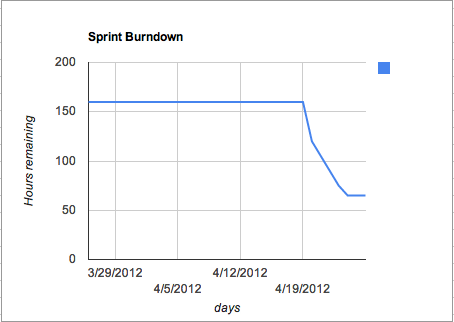
\includegraphics[width=0.8\textwidth]{images/burndown.png}
%	\caption{Burndown chart for sprint \# 2. Easter holidays and exams is the reason for the steep curve.}
%\end{figure}
The project backlog and the graph with the hours we spent are at the end of this document in appendix \ref{sec:Scrum Material}. The reader should note that the graph are vector graphics, so zooming is posible. \\
As can be seen from our backlog we have added some user stories and kept on working on some from the previous sprint.
\subsection{User Stories}
For sprint \# 2 we had the following user stories: \\
As an analytic \\
I want to make pie charts, column charts, bar charts, etc \\
So that I can make data more presentable \\

As an analytic \\
I want to make charts interactive  \\
So that I can make data more presentable \\

As an analytic \\
I want a way to show selected data from the chart \\
So that I can make data more presentable\\

As an analytic \\
I want to save data for later sessions \\
So I can continue working on datasets \\

\subsection{Tasks} % (fold)
\label{sub:Tasks}
We divided the stories up in the following tasks
% subsection Tasks (end)Tasks
\begin{itemize}
	\item Research testing tools for Sencha/JavaScript
	\item Research static code analysis tool for JavaScript
	\item Convert CSV to JSON
	\item Integrate Jstat into the app
	\item Create charting functionality
\end{itemize}










% section Sprint Material (end)
